\documentclass[twocolumn]{../cs-classes/cs-classes}

\title{Adversarial Attacks on Computer Vision Systems}
\author{Pierre-Gabriel Berlureau\and Antoine Groudiev\and Matéo Torrents}
\date{}

\addbibresource{report.bib}
\graphicspath{{../images/}}
% TODO: add more citations in the text

\begin{document}
\maketitle
\section{Introduction}
Most computer vision systems -- and in particular machine-learning and deep-learning based ones -- are vulnerable to \emph{adversarial attacks}. Adversarial images, crafted on purpose by an adversary to be misclassified by a specific vision system, are becoming a threat to vision systems used in critical applications.

We will discuss the different goals that adversaries can achieve, the information that different adversarial techniques require, and provide a few examples of applications, attacks algorithms, and defence mechanisms.

\section{Adversarial attacks: taxonomy and goals}
% Intro
%
% Transferability
\subsection{Adversarial goals}
Different types of attacks might have different \emph{goals} \cite{chakraborty2021survey}, that determine the difficulty of the attack. The easiest type of attack would be \emph{confidence reduction}, in which the adversary tries to reduce the
confidence of prediction for a specifically crafted image. The most classical -- and hardest -- goal of an attack is \emph{source/target misclassification}: given an image $X$ of class $c_1$, the adversary tries to create an image $X^*$, visually similar to $X$, but classified by the model as class $c_2\neq c_1$. For instance, an attacker might want to alter a \say{stop} sign image in such a way that the resulting image is classified by an autonomous vehicle system as a \say{priority} sign. This is usually done by adding a small variation $\delta X$ to the original image, such that $X^*=X+\delta X$ is misclassified while maintaining $\delta X$ small to avoid human detection of the attack.

\begin{figure}[H]
    \centering
    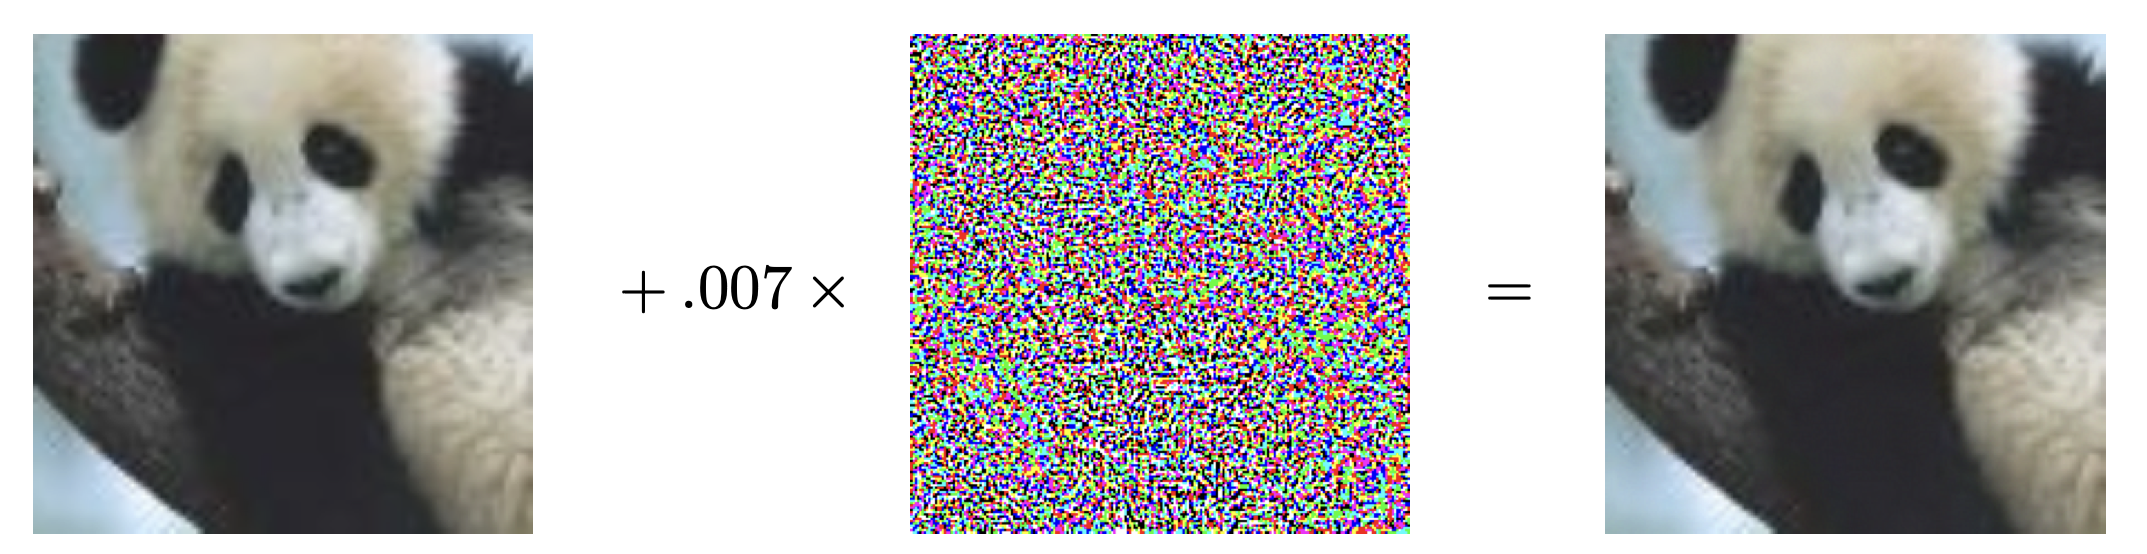
\includegraphics[width=\linewidth]{panda.png}
    \caption{Example of an adversarial image.\cite{goodfellow2014explaining} The image on the left is classified as a panda with high confidence by the model, while the image on the right is classified as a gibbon.}
\end{figure}

\subsection{Adversarial capabilities}
The term \emph{adversarial capabilities} is used to describe the different types of information that an adversary knows about the vision system \cite{chakraborty2021survey}. The quantity of information available to the attacker directly determines the difficulty of the task, and shapes the form that an attack might take.

\subsubsection{Training v. testing phase approaches}
Two main paradigms of attacks are to be distinguished. \emph{Training phase} approaches manipulate the samples and labels used during training, corrupting the system directly by altering the dataset.

Nevertheless, most attacks are \emph{testing phase} approaches, where an image is fed to the model without control over its parameters. These attacks can either be \emph{white-box} or \emph{black-box} methods, depending on the knowledge the attacker has of the trained model.

\subsubsection{White-box v. black-box approaches}
In the \emph{white-box} setup, the attacker has full access to a copy of the model, in particular to its internal structure. The attacker knows the type of model (for instance, a CNN with given architecture), the parameters of the model (for instance, the weight matrices), and has the ability to both query the model and differentiate it when it makes sense. This is by far the strongest setup for adversarial attacks, making open-source models easy targets for attacks.

The \emph{black-box} setup is less permissive. The attacker might only have access to the model as an oracle, with the possibility to query the label for a specific input image. Even weaker strategies have only at their disposal a set of pre-queried tuples $(x, y)$ of input images and labels. In both cases, a common black-box approach is to train a surrogate model using the queried examples, and to apply white-box algorithms on it.

\begin{figure*}[t]
    \centering
    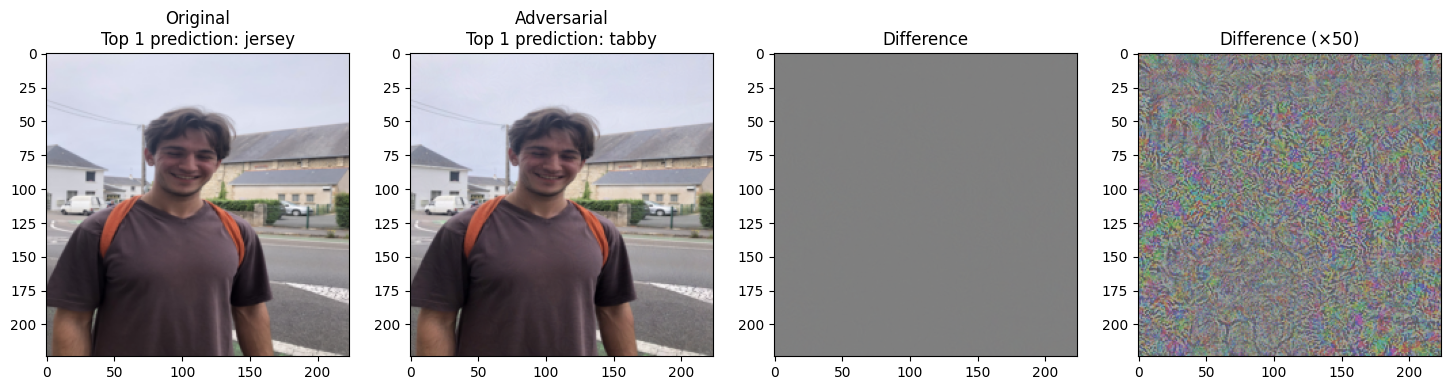
\includegraphics[width=\linewidth]{fgsm-tabby.png}
    \caption{Iteration of FGSM to misclassify an image as \texttt{tabby}\\(model: \texttt{ResNet-18}; iterations: 6; $\alpha=0.001$)}
    \label{fig:fgsm-pg}
\end{figure*}
\subsection{Real-world examples}
It has been shown that lack of robustness of widely-used vision systems can be used with malicious intents in multiple real-world situations. For instance, biometric identification systems can be fooled into classifying a person as another. Modified street signs can cause major damage on autonomous vehicles by taking control over their perception space. Slightly modified license plates can allow an attacker to become invisible to automatic parking controls, without adding any meaningful pattern to the human eye.

\section{Attacks algorithms}
\label{sec:attacks-algorithms}
We now introduce a few selected algorithms to build adversarial images. Such methods have the upsides of being both easy to understand and implement, and extremely effective on unprotected systems.

\subsection{Fast Gradient Sign Method (FGSM)}
The Fast Gradient Sign Method (FGSM) \cite{goodfellow2014explaining} goal is \emph{confidence reduction}. It calculates the effect of a variation of the input in a single step using the gradient of the cost function of the system, with respect to the input; the objective is therefore to maximize the loss. Such an attacked image is computed as follows:
\begin{equation*}
    X_* = X + \epsilon\sign\left(\nabla_x J(X, y_{\text{true}})\right)
\end{equation*}
where $J$ denotes the loss function and the parameter $\epsilon$ controls the amplitude of the changes.
This method is extremely simple to implement for a deep neural network in a white-box setup, as the gradient of the loss can be computed using backpropagation. Images are generated quickly (only one iteration), and are guaranteed to be undetectable for a small enough $\epsilon$.

Note that FGSM can be adapted for \emph{source/target misclassification}. Given a target class $y_{\text{target}}$, one can build:
\begin{equation*}
    X_* = X - \epsilon\sign\left(\nabla_x J(X, y_{\text{target}})\right)
\end{equation*}
to maximize the confidence for $y_{\text{target}}$ -- hence the minus sign.

Although this technique is already very efficient, it can be enhanced by going through multiple steps of gradient evaluation and using a smaller step size. This usually leads to smaller and more precise perturbations -- as one can stop as soon as the input is misclassified.

An implementation of this method is provided along with the report, and the results are show in \autoref{fig:fgsm-pg}.

\subsection{Facial accessories}
As opposed to digital attacks -- such as FGSM -- which require the attacker to have direct digital access to the image fed into the model, physical attacks \cite{kurakin2018adversarial} aim at fooling the model without such control over the input. For instance, dodging attacks (causing the model to misclassify a face as any other face) and impersonation attacks (causing the model to misclassify a face as a specific target) can be performed on facial recognition systems by wearing maliciously crafted accessories such as eye-glasses. While randomly colored eye-glasses can already effectively perform a dodging attacks, color patterns can be fine-tuned to perform impersonation attacks. It has been shown that such attacks can be performed with a high success rate, even in a black-box setup, using particle swarm optimization algorithms \cite{sharif2016accessorize}.
\begin{figure}[H]
    \centering
    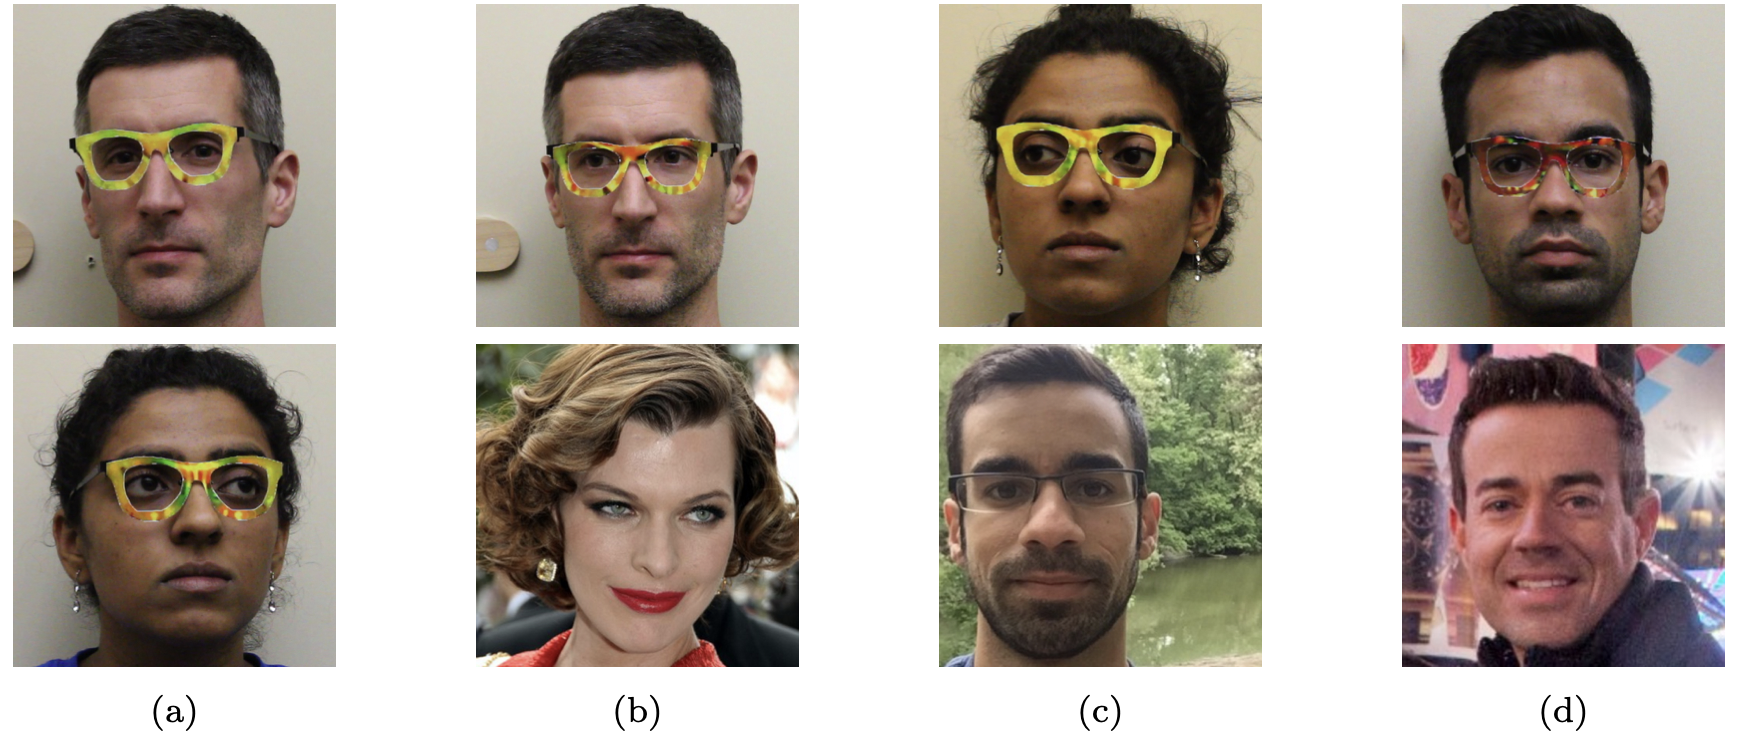
\includegraphics[width=\linewidth]{facial-accessories.png}
    \caption{Facial accessories used to fool facial recognition systems \cite{sharif2016accessorize}}
\end{figure}


\begin{figure*}
    \centering
    \renewcommand{\arraystretch}{1.2}
    % \resizebox{1\textwidth}{!}{
    \begin{tabular}{|p{3.7cm}||c|c|c|c|}
      \hline
      \centering Defense & Real data acc. & Adv. acc. $\epsilon=0.1$ & $\epsilon=0.5$ & $\epsilon=1$\\
      \hline\hline
      None & 98.90\% & 96.86\% & 69.06 & 21.07\%\\\hline
      Adversarial training & 98.99\% & 95.27\% & 86.82\% & 94.28\%\\\hline
      \texttt{NULL} labeling & 98.97\% & 100\% & 100\% & 100\% \\\hline
    \end{tabular}
    % }
  \caption{Experiments done on a CNN trained on the \texttt{MNIST} dataset.}
  \label{fig:defense-comparison}
\end{figure*}
\section{Defence mechanisms}
As the threat of adversarial images for computer vision systems increases, recent literature introduced diverse practical defence mechanisms. Nevertheless, it is worth knowing that defence remains an extremely challenging task; the lack of mathematical tools to model adversarial attacks makes it hard to argue that a certain mechanism will be efficient against a class of attacks.

\subsection{Adversarial training}
A simple and standard defence strategy is to increase the robustness of the vision system by training the model on adversarial examples. This can be done by training the model with legitimate examples as well as crafted adversarial examples. Another approach \cite{goodfellow2014explaining} consists in modifying the loss function:
\begin{multline*}
    \tilde{J}_\theta(x, y) = \alpha J_\theta(x, y) \\+ (1-\alpha)J_\theta\left(x+\epsilon\sign\left(\nabla_x J_\theta(x, y)\right)\right)
\end{multline*}
This would force the model to predict the same class for both the original and the modified image -- in this case crafted using FGSM.

\subsection{\texorpdfstring{\texttt{NULL}}{NULL} labeling}
Another defence approach is to allow the vision model to reject adversarial examples. Such a training procedure can take the following form:
\begin{enumerate}
    \item Train a classifier on clean images.
    \item Introduce a new \texttt{NULL} label, compute adversarial examples using the clean dataset with different amplitudes, and assign to each a \texttt{NULL} probability depending on this amplitude.
    \item Continue to train the classifier on both the clean and adversarial images.
\end{enumerate}
Instead of classifying adversarial examples as the original label -- which is a hard task -- we instead train the model to recognize adversarial examples. This allows to reject adversarial examples without lowering the performance of the model on legitimate data. Such an approach is considered to be the most efficient defence mechanism to date \cite{chakraborty2021survey}.

An implementation of both methods is provided along with the report, and comparison of the results of these two defence mechanisms is shown in \autoref{fig:defense-comparison}.

\section{Conclusion}
Simple yet effective methods allow attackers to fool highly accurate computer vision systems, by optimizing images in such a way that they are misclassified yet undetectable from the original to the human eye. While this causes a major threat to vision systems used in real-world, critical systems, the defence mechanisms introduced to this day do not provide a complete protection to such attacks.

% \vfill\null
\nocite{*}
\printbibliography

\end{document}